\documentclass[10pt, a4paper]{article}

% On écrit en français
\usepackage[utf8]{inputenc}
\usepackage[frenchb]{babel}
\usepackage[T1]{fontenc}

% Packages nécessaires
\usepackage{graphicx}
\usepackage{hyperref}

% Numérotation de page custom
\usepackage{fancyhdr}
\usepackage{lastpage}
\pagestyle{fancy}
\fancyhf{}
\rfoot{Page \thepage \hspace{1pt} sur \pageref{LastPage}}

% Police Helvetica <3
\usepackage{helvet}
\renewcommand*{\familydefault}{\sfdefault}

% Enlever les alinéas
\setlength{\parindent}{0pt}

% Marges plus larges pour faire moins LaTeX
\usepackage[left=3cm, right=3cm]{geometry}

% Sous titre de document
\usepackage{titling}
\newcommand{\subtitle}[1]{%
  \posttitle{%
    \par\end{center}
    \begin{center}\large#1\end{center}
    \vskip0.5em}%
}

% En tête complet de document
\newcommand{\Document}[1]{%
    \title{#1}
    \subtitle{Dématérialisation d'un processus de paiement}
    \author{
        COMETS Jean-Marie \\
        DELMARRE Adrian \\
        REYNOLDS Nicolas \\
        TURPIN Pierre
    }
    \date{\today}

    \maketitle \newpage

    \tableofcontents \newpage
}


\begin{document}

\Document{Architecture applicative}

\section{Définition des objets métiers}
La figure \ref{fig:mcd} est le MCD (Modèle Conceptuel de Données) global du
système. Il recense toutes les données utilisées dans le système d'information
de l'étude. \\

\begin{landscape}
  \begin{figure}[ht]
      \centering
      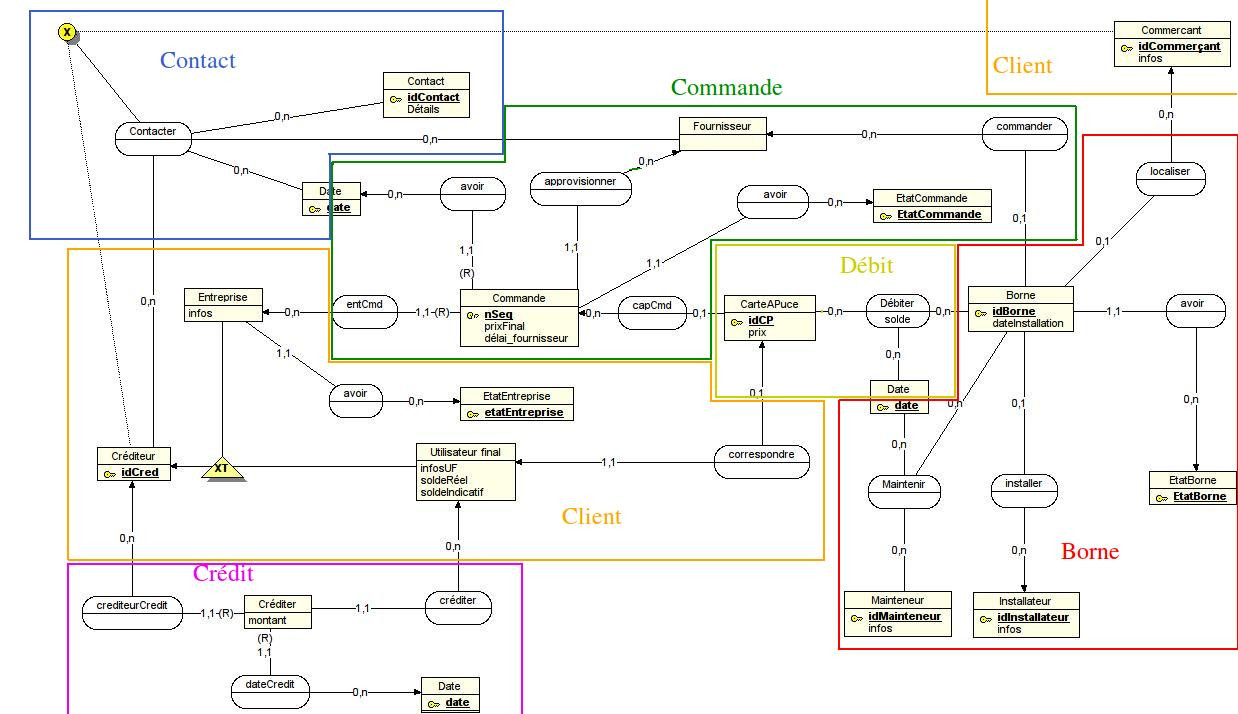
\includegraphics[width=0.7\paperheight]{mcd}
      \caption{MCD global du système}
      \label{fig:mcd}
  \end{figure}
\end{landscape}

Les objets métiers utilisés dans la solution sont les suivants : \\
\begin{description}
  \item[Contact] ...
  \item[Date] ...
  \item[Commande] ...
  \item[Carte à puce] ...
  \item[Borne] ...
  \item[Etat d'une borne] ...
  \item[Fournisseur] ...
  \item[Commercant] ...
  \item[Etat d'une commande] ...
  \item[Entreprise] ...
  \item[Etat d'une entreprise] ...
  \item[Créditeur] ...
  \item[Utilisateur final] ...
  \item[Mainteneur] ...
  \item[Installateur] ...
\end{description}

\section{Extraction des blocs fonctionnels}
A partir du MCD \ref{fig:mcd}, 6 blocs fonctionnels ont été retenu :
\begin{itemize}
  \item Contacts
  \item Clients
  \item Débit
  \item Crédit
  \item Commande
  \item Borne
\end{itemize}
~\\

% TODO dire comment les BF ont été obtenu

\subsection{Contacts}
% TODO commentaire

\subsection{Clients}
% TODO commentaire

\subsection{Débit}
% TODO commentaire

\subsection{Crédit}
% TODO commentaire

\subsection{Commande}
% TODO commentaire

\subsection{Borne}
% TODO commentaire

\section{Listing des applications utilisateurs}
Le découpage applicatif le plus pertinent est un découpage par type de client.
Les usages sont variés en fonction de l’acteur, et cela donne au client une
interface unique. Egalement, les règles de suivi varient d’un acteur à
l’autre.\\

Nous avonc alors 3 acteurs principaux dans l'étude ce qui donne 3 applications
utilisateurs : \\
\begin{itemize}
  \item Application de gestion d'un commerçant
  \item Application de gestion d'une entreprise
  \item Application de gestion d'un utilisateur final
\end{itemize}
~\\

\CUBref
{Application de gestion d'un commerçant}
{
  Cette application permet principalement aux commerçant de gérer et visualiser
  leurs transactions effectuées en utilisant ce système. \\

  Il permet également aux commerçant de signaler si un problème à eu lieu
  durant l'utilisation du système, ou si il y a eu une erreur après
  l'utilisation. \\
}
{Commerçant}
{
  Le commerçant doit être inscrit comme un commerçant auprès d'Aventix et donc
  avoir une ou plusieurs bornes. \\

  Les actions qu'il peut effectuées sont disponible uniquement grâce à une
  identification sur l'IHM des services métiers correspondants (sauf mention
  contraire explicite sur un des services métier). \\

  Les identifiants à fournir pour s'authentifier sont établies durant
  l'enregistrement du commerçant dans le SI. \\
}
{Pas de conséquences}
{
  \begin{itemize}
    \item Le commerçant n'est pas authentifié lorsqu'il essaye d'utiliser un
      service nécessitant une authentification. Il est alors simplement redirigé
      vers la connexion.
  \end{itemize}
}

\CUBref
{Application de gestion d'une entreprise}
{
  Cette application permet principalement aux entreprises de gérer leurs
  employés en tant qu'utilisateurs finaux dans le SI. \\

  L'entreprise peut effectuer des requêtes pour créer ou supprimer un
  utilisateur. \\

  Il peut aussi décider de désactiver un de ses employées temporairement ce qui
  permet de gérer les cas où les titres-restaurant sont pas utilisables (en
  vacances par exemple). L'entreprise a, bien sur, la possibilité de réactiver
  un de ses employés. \\

  L'ajout de crédits mensuelles dans les comptes de ses employés est à la
  charge de l'entreprise. Elle possède donc un moyen de créditer ses propres
  employés. \\

  Il permet également aux entreprises de signaler si un problème à eu lieu
  durant l'utilisation du système. \\
}
{Entreprise}
{
  L'entreprise doit être inscrit comme une entreprise auprès d'Aventix. \\

  Les actions qu'il peut effectuées sont disponible uniquement grâce à une
  identification sur l'IHM des services métiers correspondants (sauf mention
  contraire explicite sur un des services métier). \\

  Les identifiants à fournir pour s'authentifier sont établies durant
  l'enregistrement de l'entreprise dans le SI. \\
}
{Pas de conséquences}
{
  \begin{itemize}
    \item L'entreprise n'est pas authentifié lorsqu'il essaye d'utiliser un
      service nécessitant une authentification. Elle est alors simplement
      redirigé vers la connexion.
  \end{itemize}
}

\CUBref
{Application de gestion d'un utilisateur final}
{
  Cette application permet principalement aux utilisateurs finaux de gérer leurs
  crédits sur leur carte à puce. \\

  Il peuvent consulter l'état du compte de leur carte à puce. \\

  En tant que personne morale souscrivant à un service, il a le droit de
  modifier ses données personnelles enregistrées. \\

  Afin de pouvoir utiliser la carte à puce en dehors des limites de crédits
  imposées par son entreprise, l'utilisateur final peut se créditer lui-même. \\

  L'application permet également aux utilisateurs finaux de signaler si un
  problème à eu lieu durant l'utilisation du système. \\
}
{Utilisateur final}
{
  L'utilisateur doit être inscrit et actif auprès d'Aventix. \\

  Les actions qu'il peut effectuées sont disponible uniquement grâce à une
  identification sur l'IHM des services métiers correspondants (sauf mention
  contraire explicite sur un des services métier). \\

  Les identifiants à fournir pour s'authentifier sont établies durant
  la création de l'utilisateur final par l'entreprise dans le SI. \\
}
{Pas de conséquences}
{
  \begin{itemize}
    \item L'utilisateur final n'est pas authentifié lorsqu'il essaye d'utiliser
      un service nécessitant une authentification. Il est alors simplement
      redirigé vers la connexion.
  \end{itemize}
}

\section{Génération des services}
\subsection{Services applicatif}
La liste des services applicatifs est la suivante : \\
\begin{itemize}
  \item Application de gestion d'un commerçant
  \item Application de gestion d'une entreprise
  \item Application de gestion d'un utilisateur final
\end{itemize}
~\\

\subsection{Services métier}
% Un commerçant peut signaler une panne à Aventix. Celle-ci doivent être
% enregistrer dans le SI afin d'améliorer la qualité du produit et tracer les
% éventuelles erreurs. \\
% 
% Un commerçant à le droit de visualiser et suivre les transactions physiques
% utilisant les services de la solution. Les transactions sont enregistrées dans
% le SI et un commerçant habilité doit pouvoir avoir accès à celles-ci. \\

\subsubsection{Contacts}
\subsubsection{Clients}
\subsubsection{Débit}
\subsubsection{Crédit}
\subsubsection{Commande}
\subsubsection{Borne}

\subsection{Services objet métier}

\section{Description du workflow}
\begin{figure}
  \centering

  \begin{sequencediagram}
      \newthread{acteur}{Acteur~:~Utilisateur final}
      \newinst{ihm}{IHM}
      \newinst{sm}{SM~:~Clients}
      \newinst{som}{SOM~:~Utilisateur final}

      \begin{call}{acteur}{submit(idUF, infosUF)}{ihm}{confirmation}
          \begin{messcall}{ihm}{setInfosUF(id, infos)}{sm}
            \begin{call}{sm}{findById(id)}{som}{found}
            \end{call}
            \begin{sdblock}{IF}{found = VRAI}
              \begin{callself}{sm}{checkInfosUF(infos)}{status,~message}
              \end{callself}
              \begin{sdblock}{IF}{status = OK}
                \begin{call}{sm}{setInfos(id, infos)}{som}{}
                \end{call}
                \begin{mess}{sm}{OK, ACCEPTED}{ihm}
                \end{mess}
              \end{sdblock}
              \begin{sdblock}{ELSE}{status != OK}
                \begin{mess}{sm}{NOT OK, message}{ihm}
                \end{mess}
              \end{sdblock}
            \end{sdblock}
            \begin{sdblock}{ELSE}{found != VRAI}
                \begin{mess}{sm}{NOT OK, NOT FOUND}{ihm}
                \end{mess}
            \end{sdblock}
          \end{messcall}
      \end{call}
  \end{sequencediagram}

  \caption{Modification des informations de l'utilisateurs final}
\end{figure}

\begin{figure}
  \centering

  \begin{sequencediagram}
      \newthread{acteur}{Acteur~:~Utilisateur final}
      \newinst{ihm}{IHM}
      \newinst{sm}{SM~:~Clients}
      \newinst{som}{SOM~:~Utilisateur final}

      \begin{call}{acteur}{submit(loginInfos)}{ihm}{confirmation}
          \begin{messcall}{ihm}{loginUF(loginInfos)}{sm}
            \begin{call}{sm}{findByLoginInfos(loginsInfos)}{som}{id, found, activated}
            \end{call}
            \begin{sdblock}{IF}{found = VRAI and activated = VRAI}
              \begin{callself}{sm}{connectUF(id)}{}
              \end{callself}
              \begin{mess}{sm}{OK}{ihm}
              \end{mess}
            \end{sdblock}
            \begin{sdblock}{ELSE}{found != VRAI or activated != VRAI}
                \begin{mess}{sm}{NOT OK}{ihm}
                \end{mess}
            \end{sdblock}
          \end{messcall}
      \end{call}
  \end{sequencediagram}

  \caption{Connexion de l'utilisateur final}
\end{figure}

\begin{figure}
  \centering

  \begin{sequencediagram}
      \newthread{acteur}{Acteur~:~Entreprise}
      \newinst{ihm}{IHM}
      \newinst{sm}{SM~:~Clients}
      \newinst{som}{SOM~:~Utilisateur final}

      \begin{call}{acteur}{submit(idUF)}{ihm}{confirmation}
          \begin{messcall}{ihm}{activateUF(idUF)}{sm}
            \begin{call}{sm}{findById(idUF)}{som}{found}
            \end{call}
            \begin{sdblock}{IF}{found = VRAI}
              \begin{call}{sm}{activate(idUF)}{som}{}
              \end{call}
              \begin{callself}{sm}{notifyUF(idUF)}{}
              \end{callself}
              \begin{mess}{sm}{OK}{ihm}
              \end{mess}
            \end{sdblock}
            \begin{sdblock}{ELSE}{found != VRAI}
                \begin{mess}{sm}{NOT OK}{ihm}
                \end{mess}
            \end{sdblock}
          \end{messcall}
      \end{call}
  \end{sequencediagram}

  \caption{Activation d'un utilisateur final}
\end{figure}

\begin{figure}
  \centering

  \resizebox{!}{0.85\totalheight}{\begin{sequencediagram}
      \newthread{acteur}{Acteur~:~Entreprise}
      \newinst{ihm}{IHM}
      \newinst{sm}{SM~:~Clients}
      \newinst{som}{SOM~:~Utilisateur final}
      \newinst{api}{API~:~Banque}

      \begin{call}{acteur}{submit(infosUF)}{ihm}{confirmation}
          \begin{messcall}{ihm}{createUF(infosUF)}{sm}
            \begin{call}{sm}{findByInfos(infoUF)}{som}{found}
            \end{call}
            \begin{sdblock}{IF}{found = VRAI}
              \begin{mess}{sm}{NOT OK, ALREADY EXIST}{ihm}
              \end{mess}
            \end{sdblock}
            \begin{sdblock}{ELSE}{found != VRAI}
              \begin{callself}{sm}{checkInfosUF(infosUF)}{status, message}
              \end{callself}
              \begin{sdblock}{IF}{status = OK}
                \begin{call}{sm}{create(infosUF)}{som}{id}
                \end{call}
                \begin{call}{sm}{createAccountUF(id)}{api}{status}
                \end{call}
                \begin{sdblock}{IF}{status = OK}
                  \begin{mess}{sm}{OK}{ihm}
                  \end{mess}
                \end{sdblock}
                \begin{sdblock}{ELSE}{status != OK}
                  \begin{messcall}{sm}{remove(id)}{som}
                  \end{messcall}
                  \begin{mess}{sm}{NOT OK}{ihm}
                  \end{mess}
                \end{sdblock}
              \end{sdblock}
              \begin{sdblock}{ELSE}{status != OK}
                \begin{mess}{sm}{NOT OK}{ihm}
                \end{mess}
              \end{sdblock}
            \end{sdblock}
          \end{messcall}
      \end{call}
  \end{sequencediagram}}

  \caption{Création d'un utilisateur final}
\end{figure}

\end{document}

% vim: ft=tex et sw=2 sts=2
